\documentclass[a4paper,10pt]{article}
\usepackage[utf8]{inputenc}
\usepackage{graphicx}
\usepackage{enumerate}
\usepackage{listings}
\usepackage{multirow}
\usepackage{pdfpages}
\usepackage{amsmath}
\usepackage{amsthm}
\usepackage[margin=1.3in]{geometry}
\usepackage[backref=true,pagebackref=true,breaklinks=true,letterpaper=true,colorlinks,bookmarks=true,bookmarksnumbered=true,bookmarksopen=true,hyperfigures=true]{hyperref}
\usepackage{times}
\usepackage{textcomp}
\usepackage{fancyvrb}
% Uncomment to disallow hyphenated line breaks
\usepackage[none]{hyphenat}
\raggedright


\newcommand{\HRule}{\rule{\linewidth}{0.5mm}}
\newcommand{\eps}{\varepsilon}
\newcommand{\ssum}{\displaystyle\sum}

% MACRO DEFINITIONS
\newcommand{\developeremail}{{\tt hotspotter.ir@gmail.com}}


\begin{document}
\begin{titlepage}
    \topskip0pt
    \vspace*{\fill}

    \begin{center}

        \HRule \\[0.4cm]
        { \huge \bfseries HotSpotter User Guide}\\[0.4cm]
        \HRule \\[1.5cm]

        Jon Crall (crallj@rpi.edu)\\
        Jason Parham (parhaj@rpi.edu) \\
        Chuck Stewart (stewart@cs.rpi.edu) \\ 

        \medskip

        Department of Computer Science \\
        Rensselaer Polytechnic Institute

    \end{center}

    \vspace*{\fill}
\end{titlepage}

\DeclareRobustCommand{\cmdkey}{\raisebox{-.035em}{
\includegraphics[height=.75em]{images/command}}}

\section{Usage}  This document assumes that you have already
downloaded and installed 
the Windows or Mac version (WHAT ABOUT LINUX?) of the HotSpotter software.  It describes the basic
steps of running HotSpotter to identify individual animals, including
opening a database (or creating a new one), importing images,
selecting ROIs, querying, and naming.
The instructions
are primarily focused on the Mac version of the software, but adaptation to
the windows version is easy. Just know that the control key ({\tt Ctrl}) on windows
is equivalent to the command key ({\tt Cmd} = \cmdkey) on Mac. This guide will use the
mac notation.

    \subsection{Opening the Program}
    When HotSpotter is first run, the program prompts the user to open a
    database or create a new one.  In each succeeding run, it will start by
    opening the previous database. 

    % Macros for displaying Mac/Windows Control Keys and arrows instead of ->
    \renewcommand{\textrightarrow}{$\rightarrow$}
    %\newcommand{\textcmd}{Cmd}
    \newcommand{\textcmd}{\cmdkey}
    %[fontsize=\footnotesize,frame=single,commandchars=\\\{\}]

    To create a new database: \\
    \begin{Verbatim}[commandchars=\\\{\}]
    File \textrightarrow New Database [\textcmd+N]
    \end{Verbatim}

    \begin{center}
        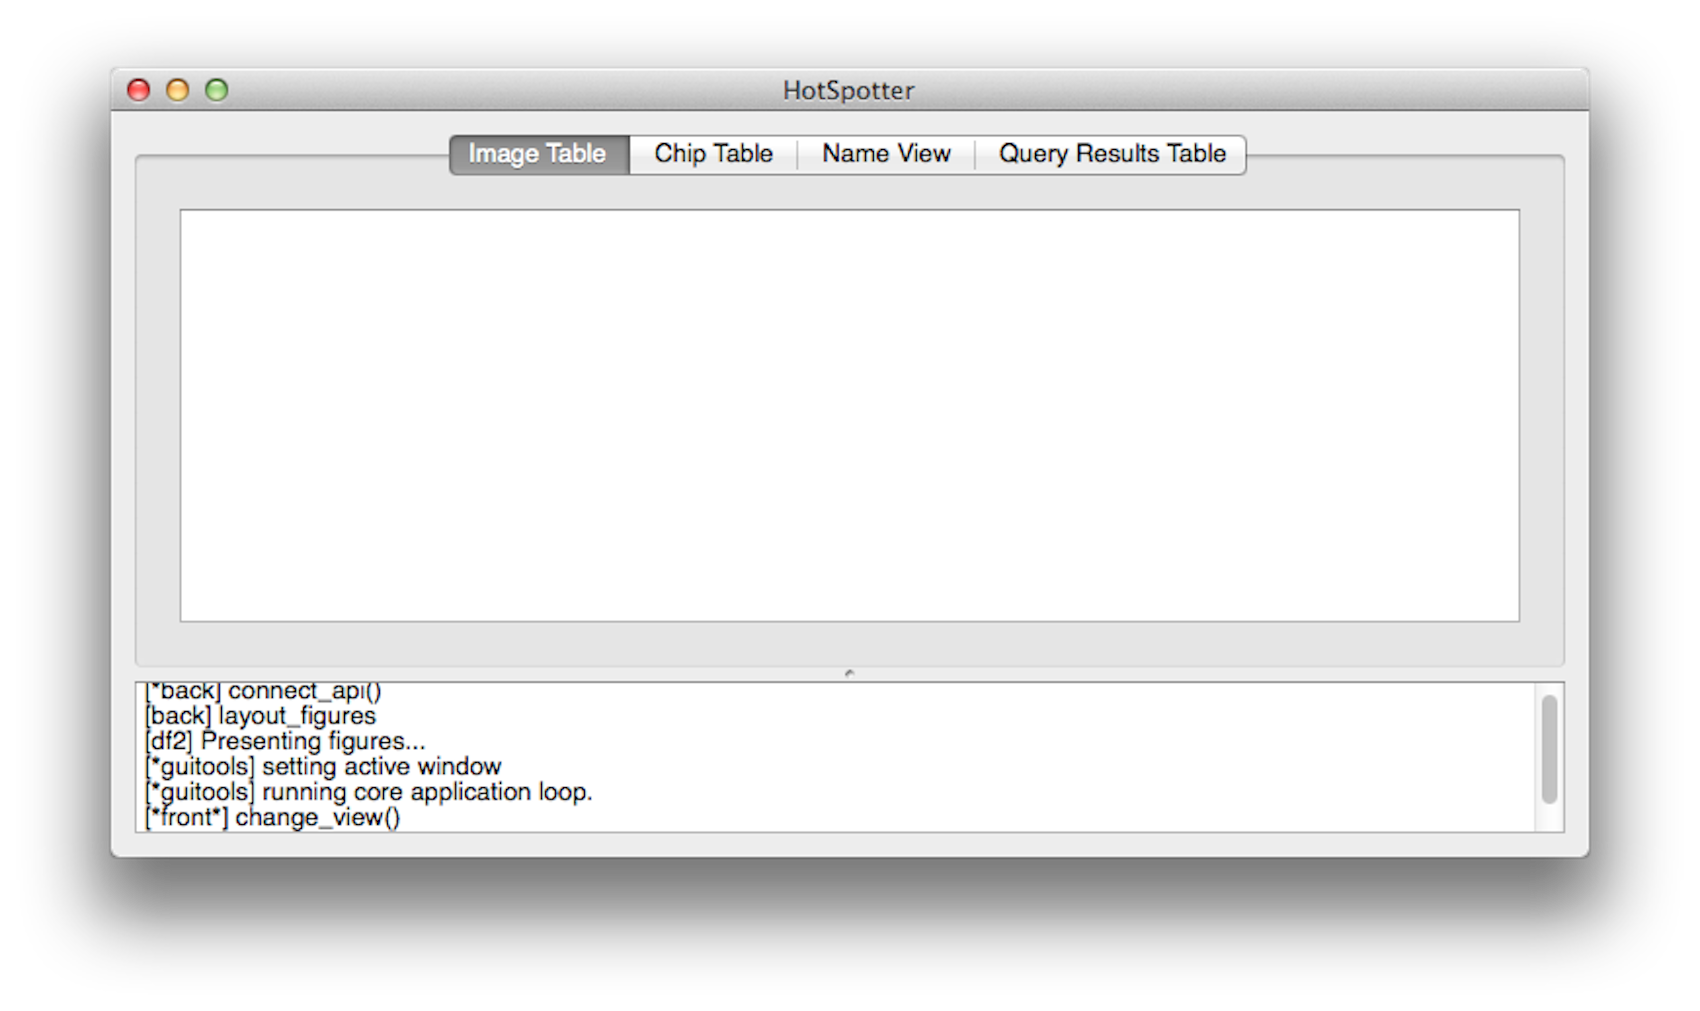
\includegraphics[scale=0.15]{images/start.png}
    \end{center}

    To open an existing database
    \begin{Verbatim}[commandchars=\\\{\}]
    File \textrightarrow Open Database [\textcmd+O]
    \end{Verbatim}


    HotSpotter can also read StripeSpotter databases by opening the
    StripeSpotter database's {\tt data} directory.  WHAT ABOUT
    PREVIOIUS VERSIONS.
    
    \subsection{Importing images}
        In order to add one or more images to the database, there are two options. To manually select specific images from a directory, there is the command
        \begin{Verbatim}[commandchars=\\\{\}]
        File \textrightarrow Import Images (select file(s)) [\textcmd+I]
        \end{Verbatim}
        There is also the option to import an entire directory of images directly into HotSpotter.  This may be achieved with the command 
        \begin{Verbatim}[commandchars=\\\{\}]
        File \textrightarrow Import Images (select directory)
        \end{Verbatim}
        \begin{center}
            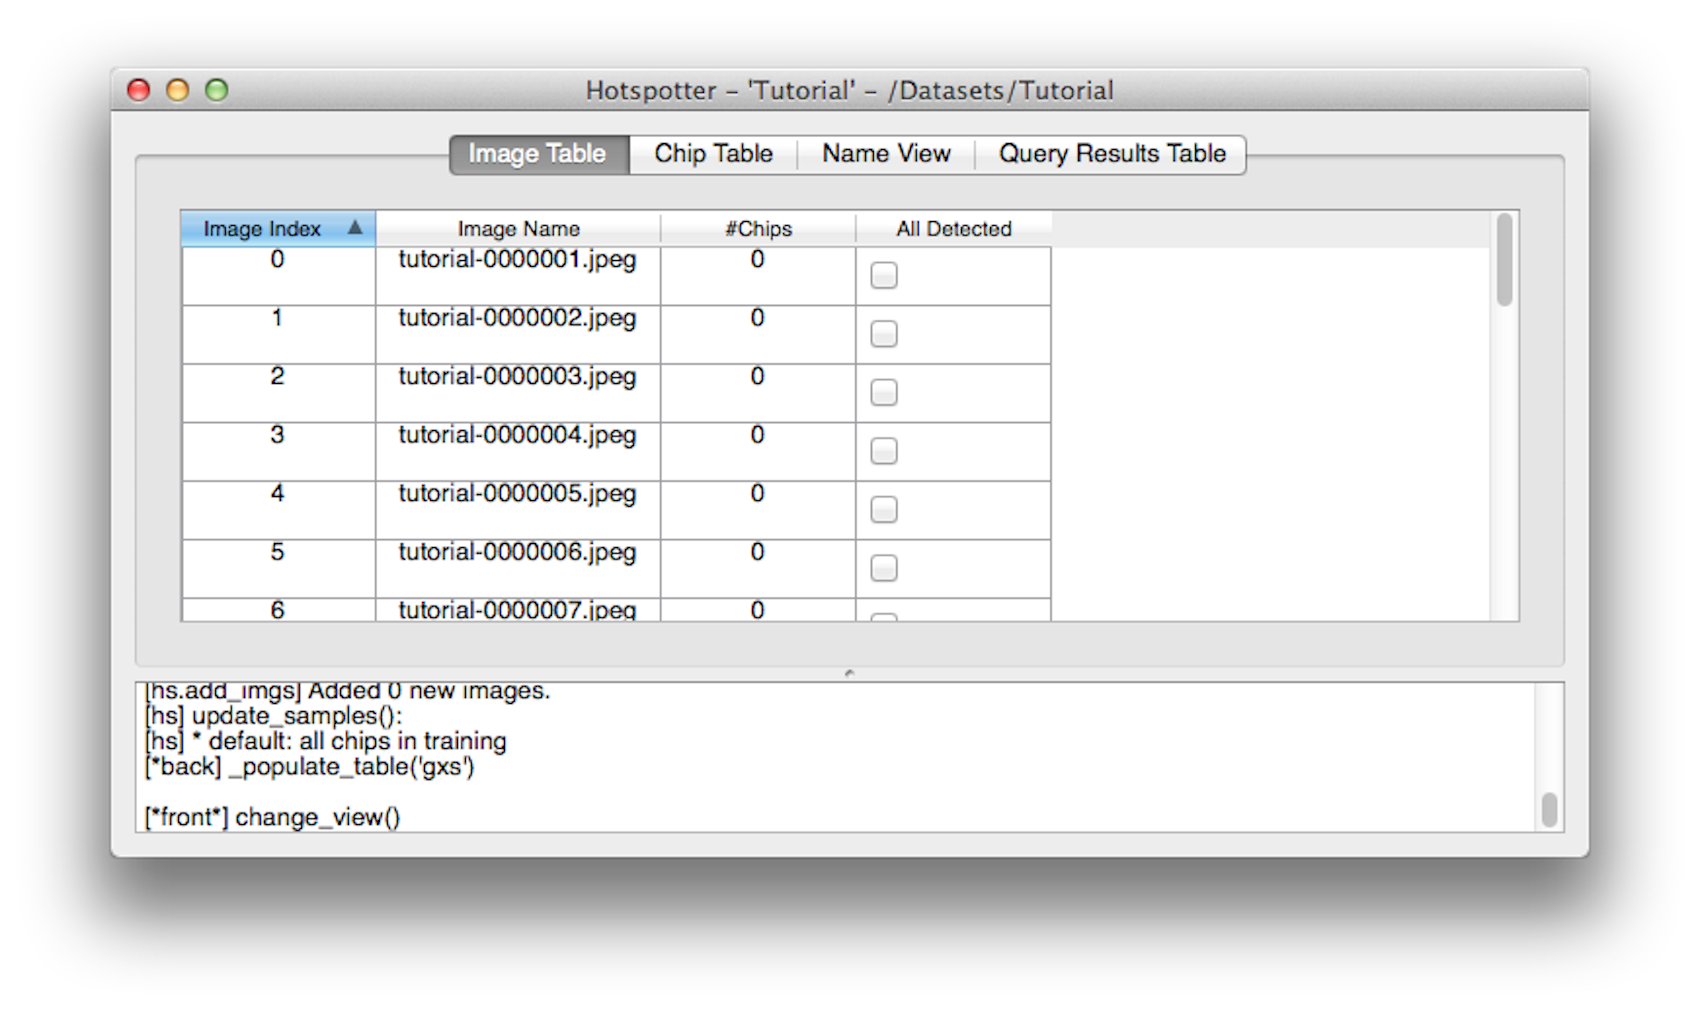
\includegraphics[scale=0.15]{images/added.png}
        \end{center}
        HotSpotter will copy all selected images into its images directory.  You may also import images by directory from the menu.
        These are automatically added to the database and may be seen under ``Image Table'

    \subsection{Defining Chips with ROIs and Orientation}
        Before using HotSpotter to identify an animal in an image ---
        or, equivalently, find other images that show the same
        animal ---- a region of interest (ROI) and an orientation must
        be assigned.  (The sub-image extracted from an ROI is called a
        ``chip''.)  The ROIs must be specified first, one for each
        animal you would like to have HotSpotter identify.
%        I REMOVED THIS NEXT PARAGRAPH.  
%        This is accomplished by
%        \begin{Verbatim}[commandchars=\\\{\}]
%        Convenience \textrightarrow Convert All Images to Chips
%        \end{Verbatim}
%        This option should be used in the relatively rare case that the
%        animal occupies almost the entire image.
%
%        The more common case is to specify the ROIs manually.  Multiple ROIs are allowed for each
%         image.  
        Each ROI should include most of the body of the animal ---
        anything that might be a distinguishing feature --- so users should err on the
        side of making the ROI too large rather than too small.

        In order to specify an ROI, the Image Table should be
        highlighted and then the image should be selected (click on
        this image).  Next, click
        \begin{Verbatim}[commandchars=\\\{\}]
        Actions \textrightarrow Add Chip [A]
        \end{Verbatim}
        and select the  ROI clicking two image points in the Image
        View to specify opposite corners of the ROI bounding box.

        \;

        If you don't like your ROI you can click on it and reselect it
        using
        \begin{Verbatim}[commandchars=\\\{\}]
        Actions \textrightarrow Reselect ROI [R]
        \end{Verbatim}
        You can use remove it entirely using 
        \begin{Verbatim}[commandchars=\\\{\}]
        Actions \textrightarrow Delete Chip
        \end{Verbatim}

        The default orientation of each chip is horizontal, and this is set
        internally by HotSpotter.  This is usually sufficient when
        taking ``normal'' pictures of standing
        animals, such as zebras or giraffes.  On the other hand, for overhead
        pictures of animals like frogs, specification of the
        orientation is \textbf{crucial for accurate recognition}.  The
        orientation is best determined by drawing an axis within the
        ROI of the animal in a way that can be repeated for each
        animal.  For frog images this is the spine.

        In order to specify an orientation other than the default
        (horizontal) orientation, the user must click
        \begin{Verbatim}[commandchars=\\\{\}]
        Actions \textrightarrow Reselect Orientation [O]
        \end{Verbatim}
        \begin{center}
            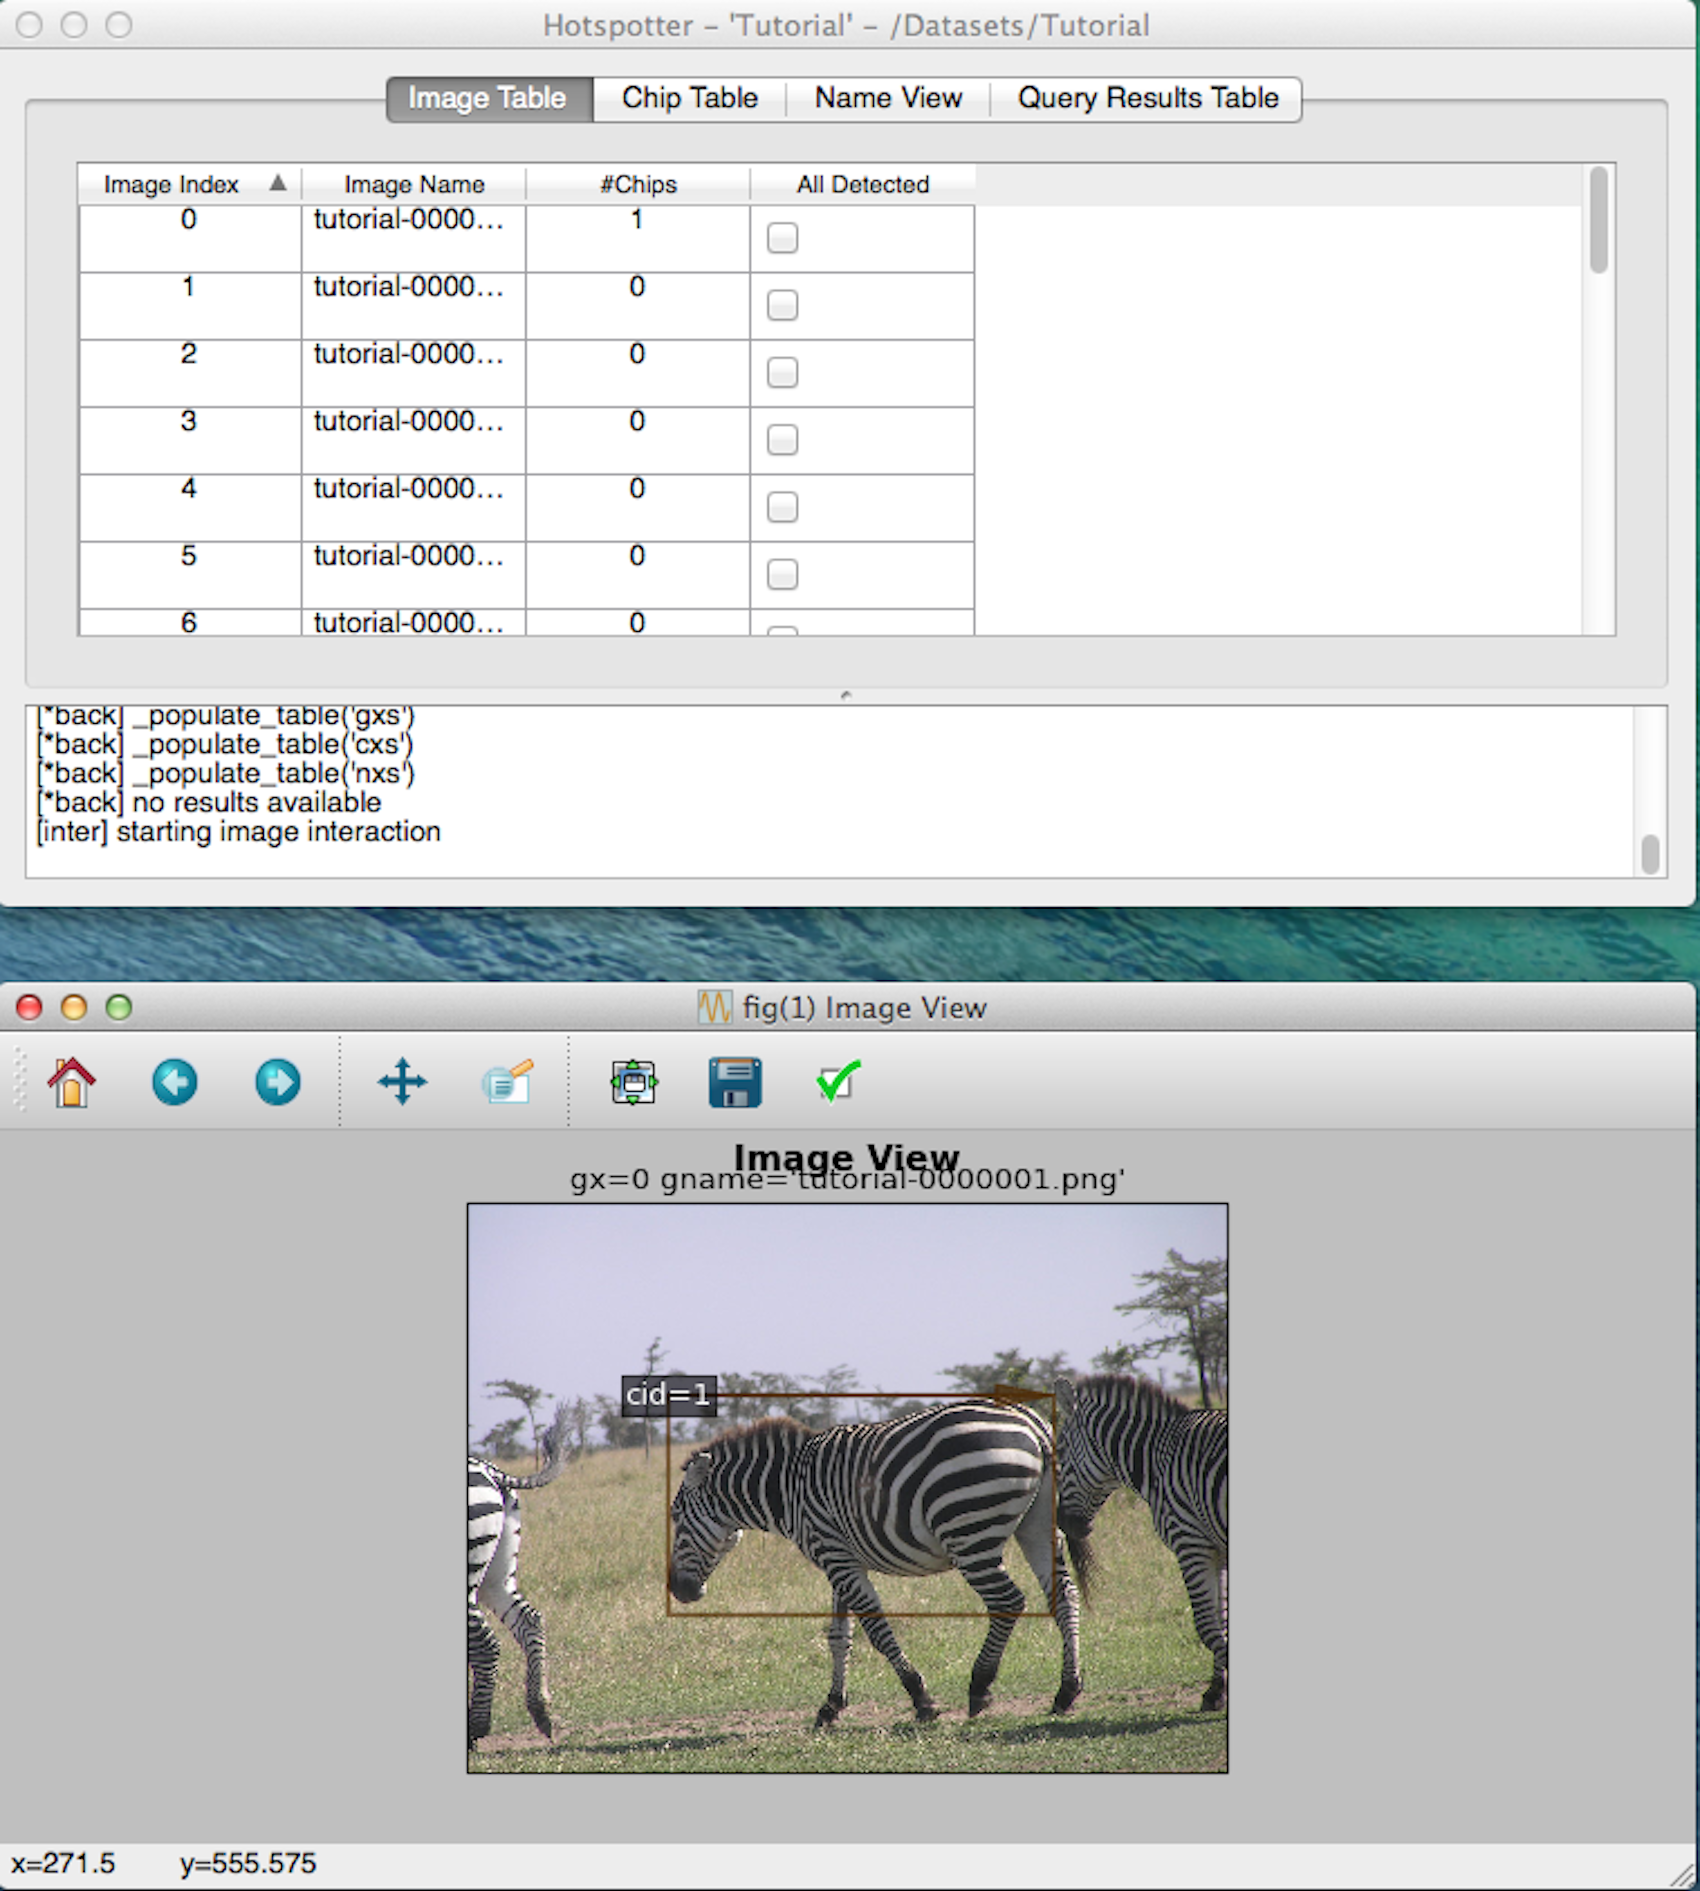
\includegraphics[scale=0.13]{images/image.png}
        \end{center}

        \noindent
        and then clicking on two points on the Image View to define
        the orientation axis.  Note that the angle does not have to be
        selected perfectly each time --- pretty close will suffice ---
        but you should be consistent with the order in which you
        click, such as first clicking on the rump and then click on
        the head.

    \subsection{Chip Properties Display (Optional)} 
        HotSpotter uses each ROI and orientation to generate a chip. 
        Within these chips HotSpotter computes its hotspots --- elliptical
        regions centered on points of interest that HotSpotter automatically
        detects.  Intuitively, the hotspots are loosely analogous to a
        part of a ``fingerprint'' for the chip.  Two chips having enough hotspot similarity
        will be matched successfully by HotSpotter. A chip can be seen by clicking 
	on the Chip Table and then selecting a chip.

        \begin{center}
          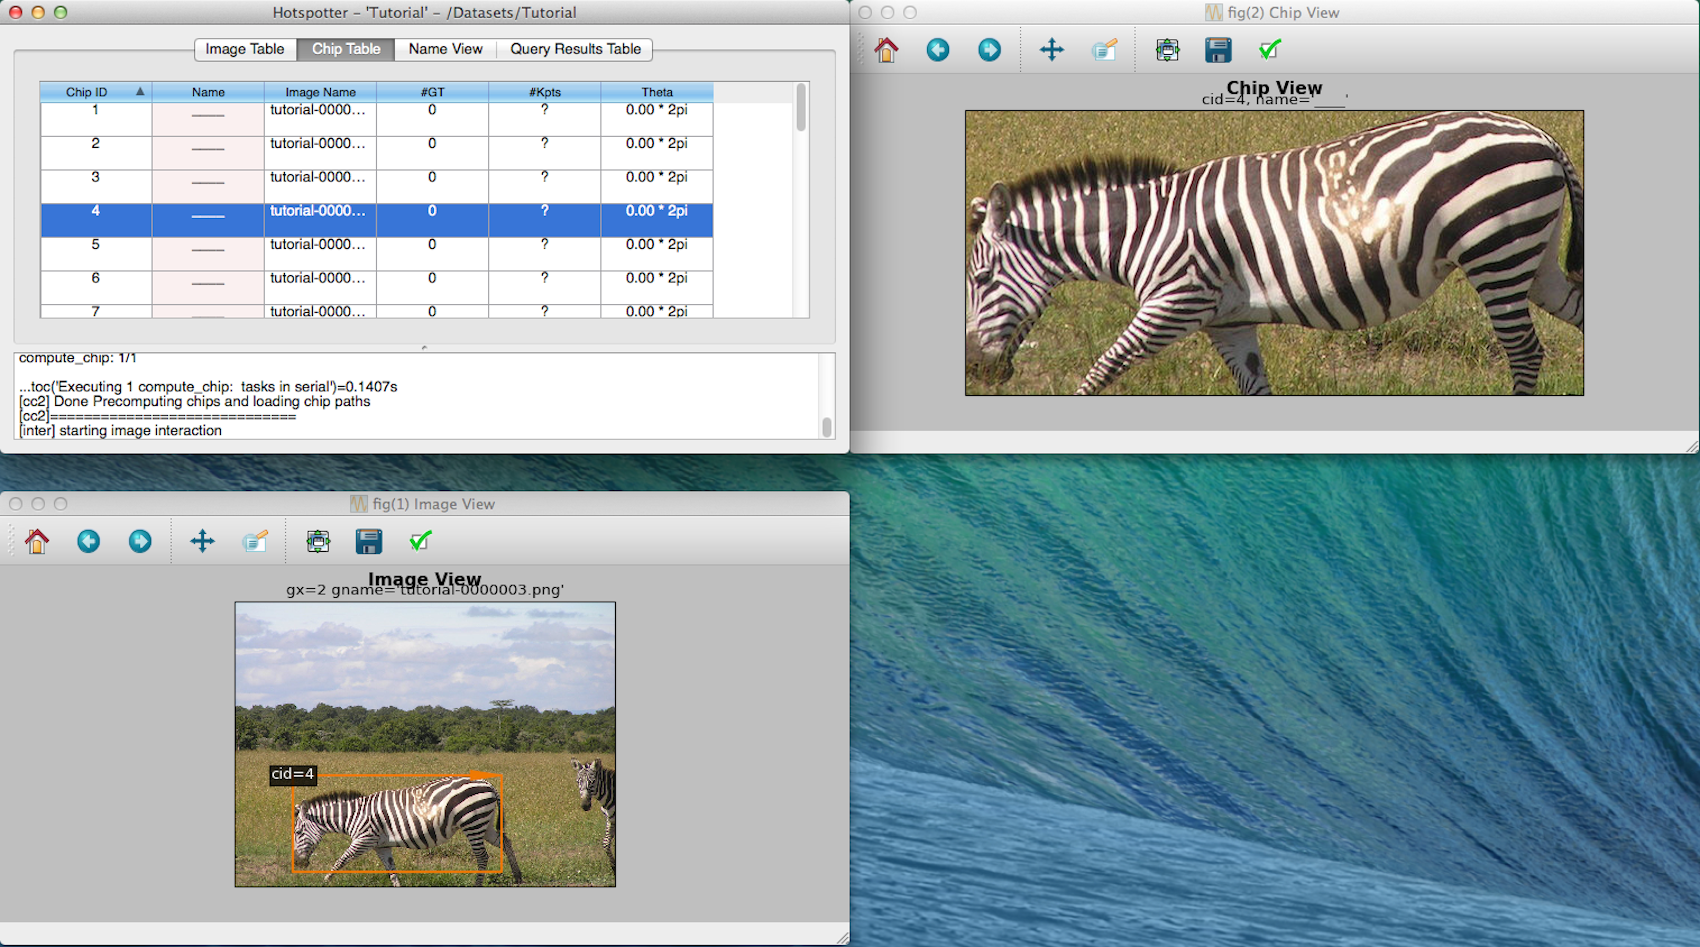
\includegraphics[scale=0.2]{images/chip.png}
        \end{center}

        The hotspots' points of interest and elliptical regions can be
        toggled on and off by clicking on the grey area around a chip in the Chip View.
	A specific hotspot can be viewed by clicking on a point of interest on the chip within the Chip View.
        \begin{center}
            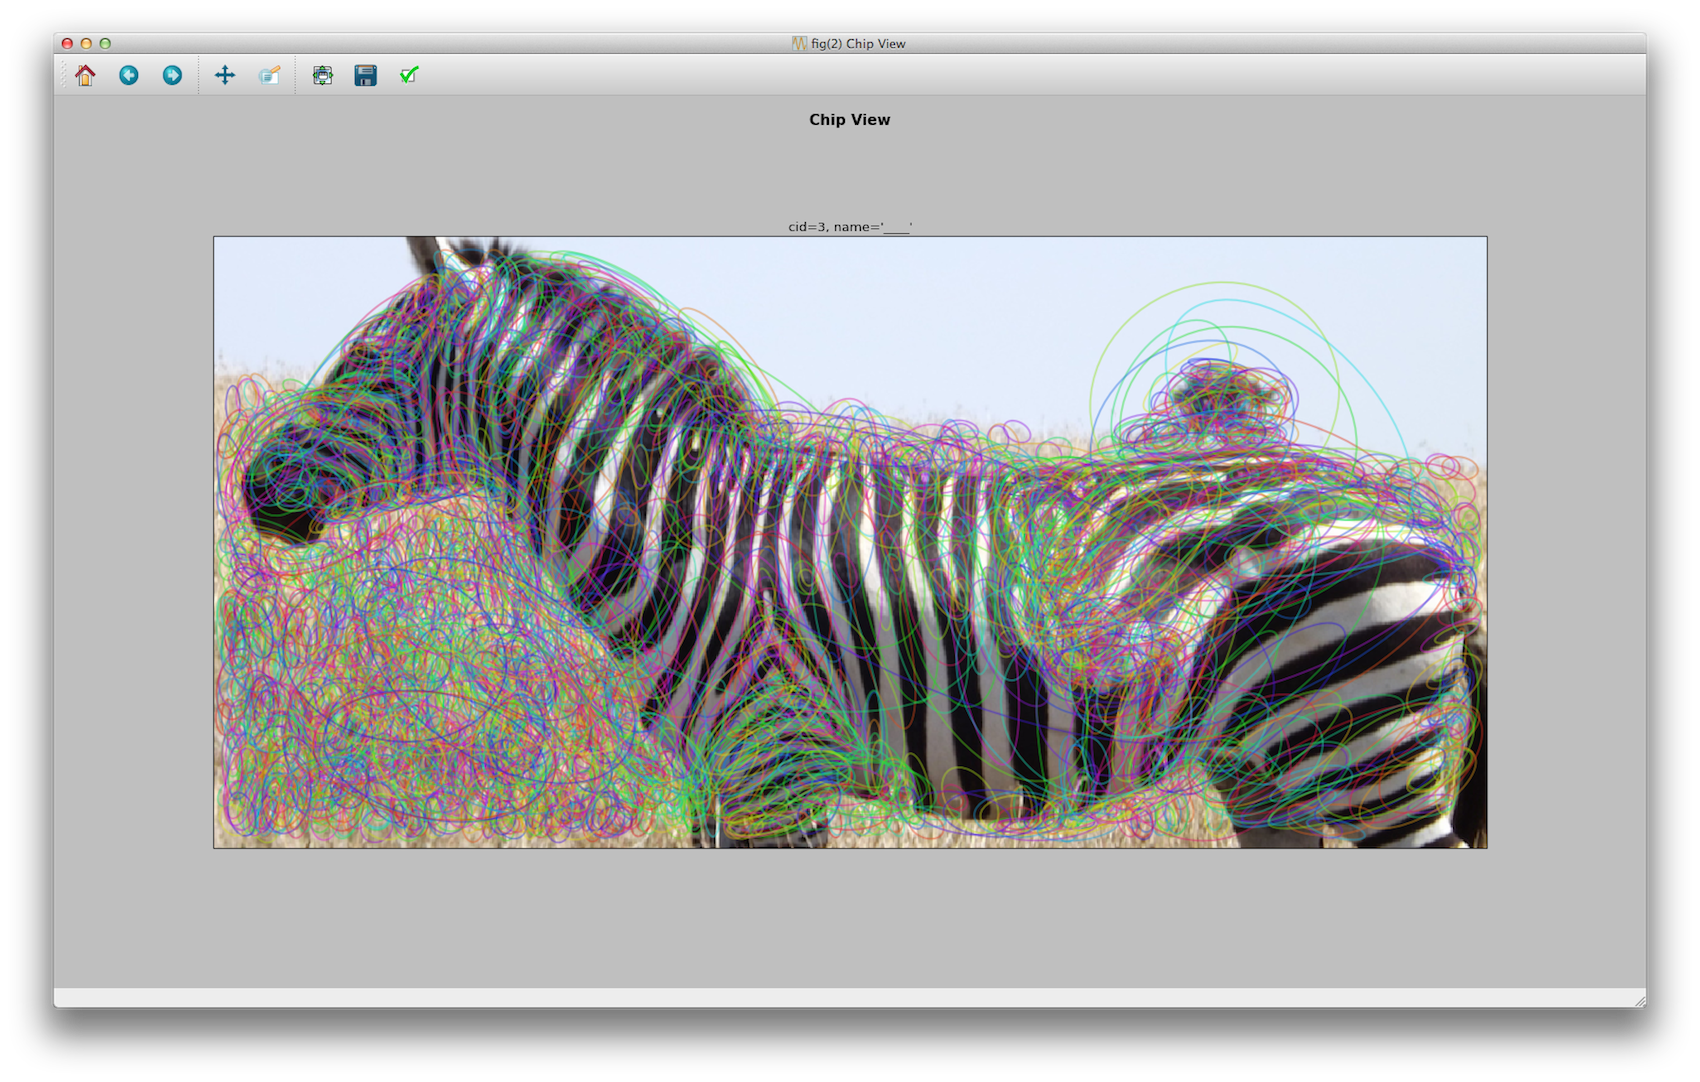
\includegraphics[scale=0.1]{images/chip-ellipse.png}
            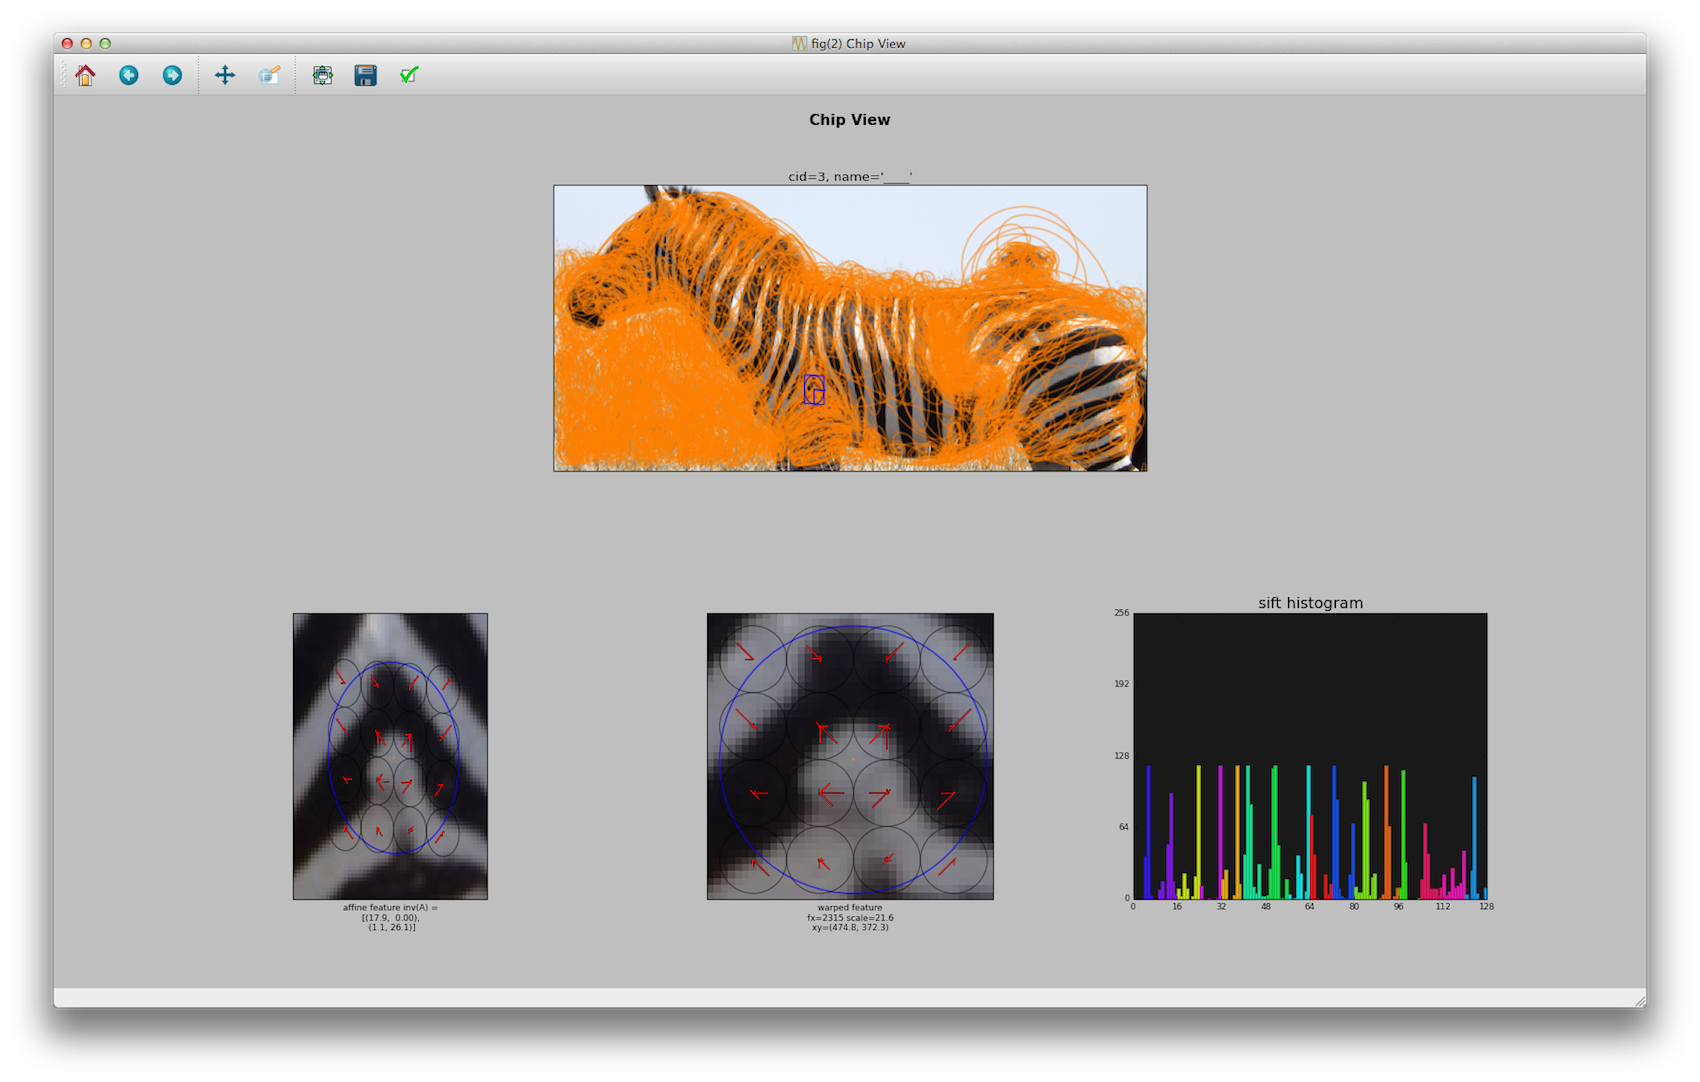
\includegraphics[scale=0.1]{images/chip-hotspot.png}
        \end{center}

        
        \begin{center}
          WHAT WAS HERE?
        \end{center}

    \subsection{Running a Query}
        A Query can be run on the selected chip.

        \begin{Verbatim}[commandchars=\\\{\}]
        Actions \textrightarrow Query [Q]
        \end{Verbatim}
        
\noindent
        This will quickly find similar chips in the database.  The program will
        automatically rank the chips in order of similarity and will highlight
        the portions of the image that it identifies as being most
        similar.

        \begin{center}
            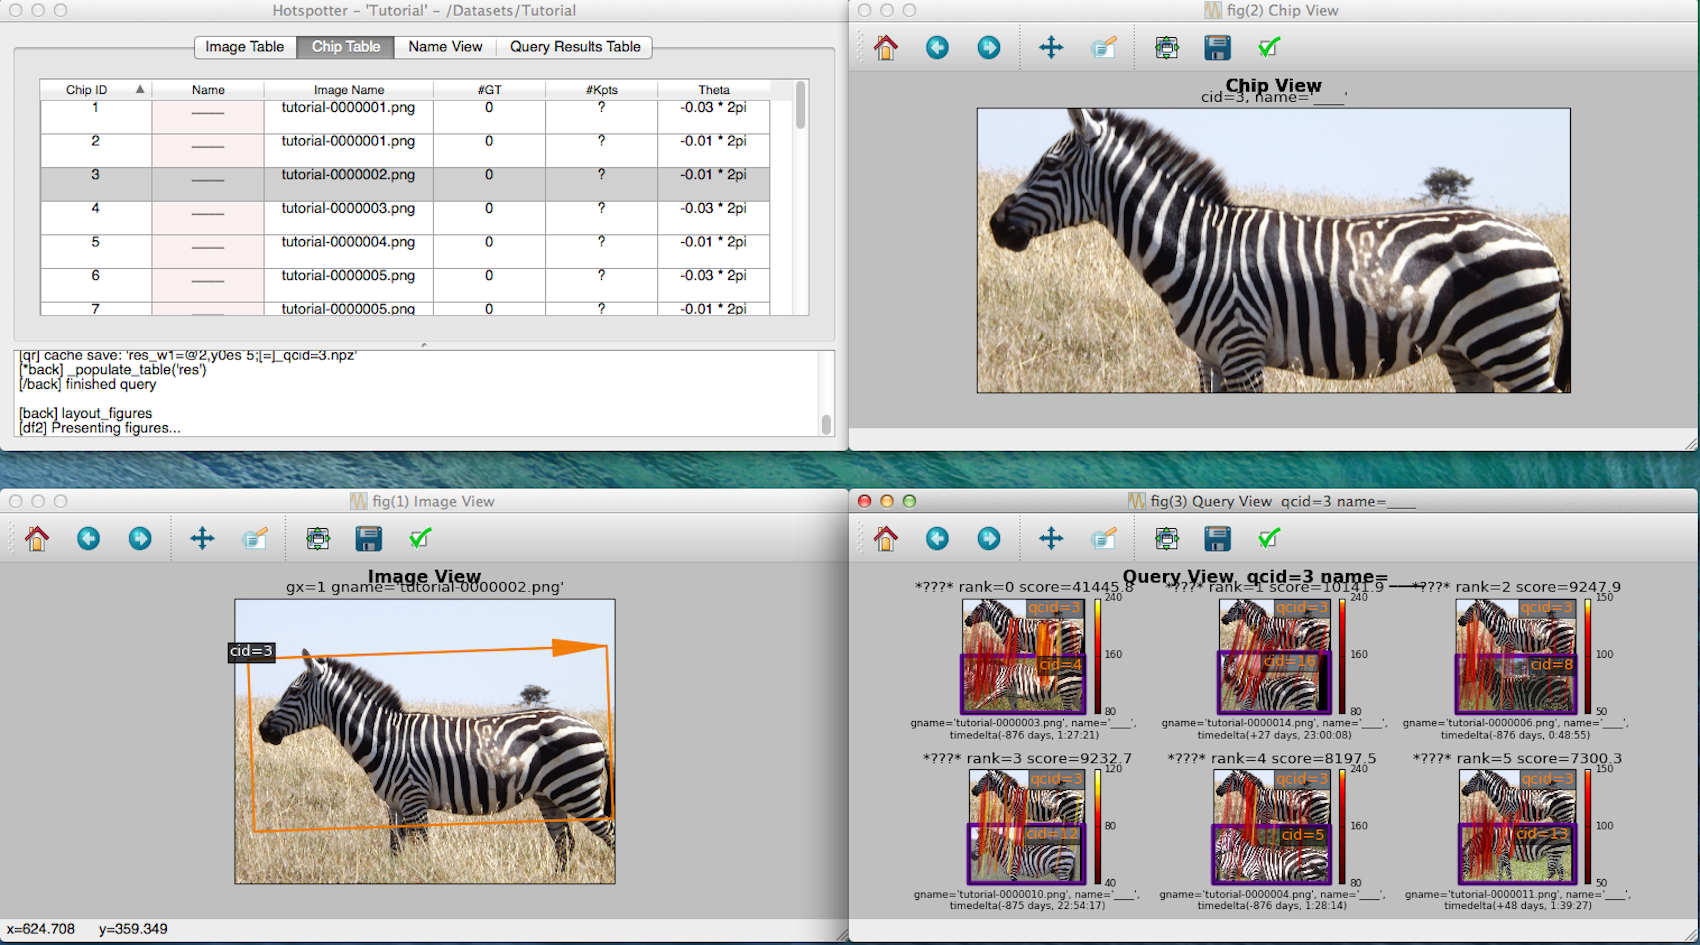
\includegraphics[scale=0.2]{images/query-all.png}

        \;

            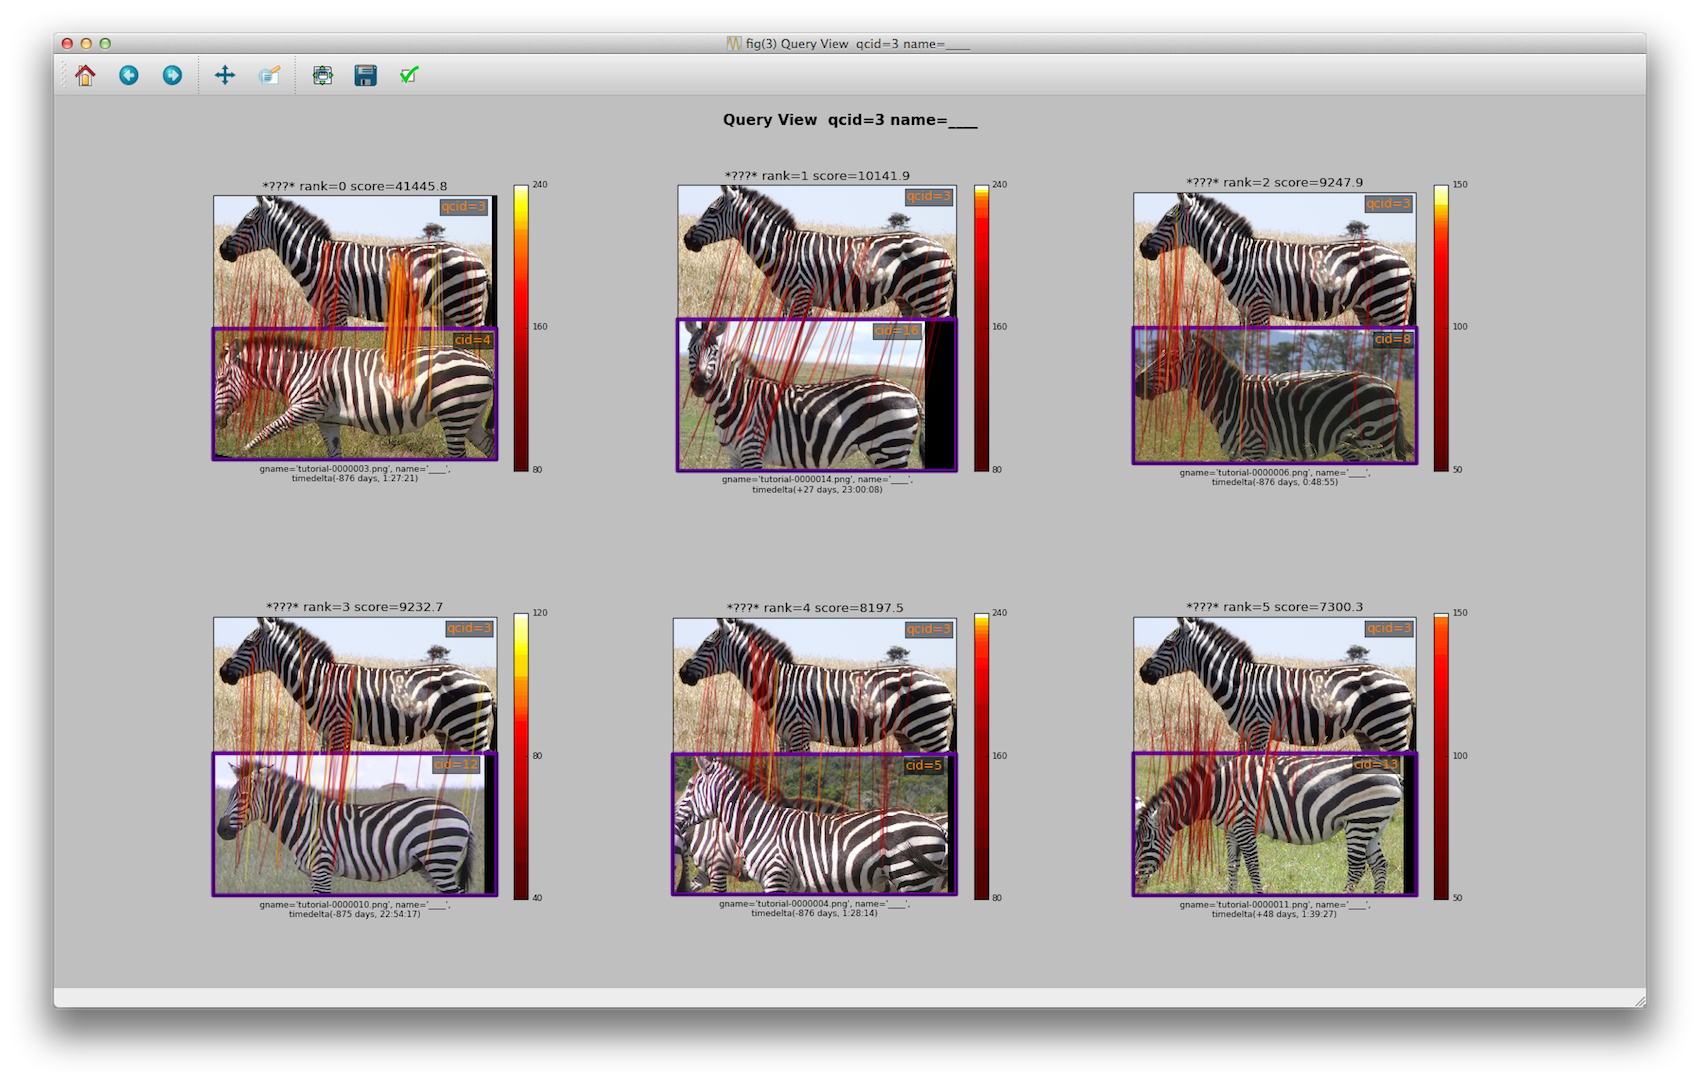
\includegraphics[scale=0.212]{images/query-result.png}
        \end{center}
        In this display, there are six results, each showing a pair of images.  In each
        pair, the query chip is shown on top and the
        potentially-matching chip is shown on the bottom.  Clicking on
        the pair will show a highlighted display.  You will also
        notice a score for each match.  The scores tend to vary a lot
        according to species and size of the image set.  Small image
        sets will produce greater scores, as will giraffes and Grevy's
        zebras. 
     
\noindent
  Once you decides based on a query that two or more chips show the
  same zebra, you record this decision by giving the chips the same
  name. This requires an understanding
  of the meaning of the names within HotSpotter, as described next.

\subsection{IDs, Names, and Recording Matching Results}

   In the Chip Table, users will see Chip ID, Name, and Image Name columns.

\begin{center}
            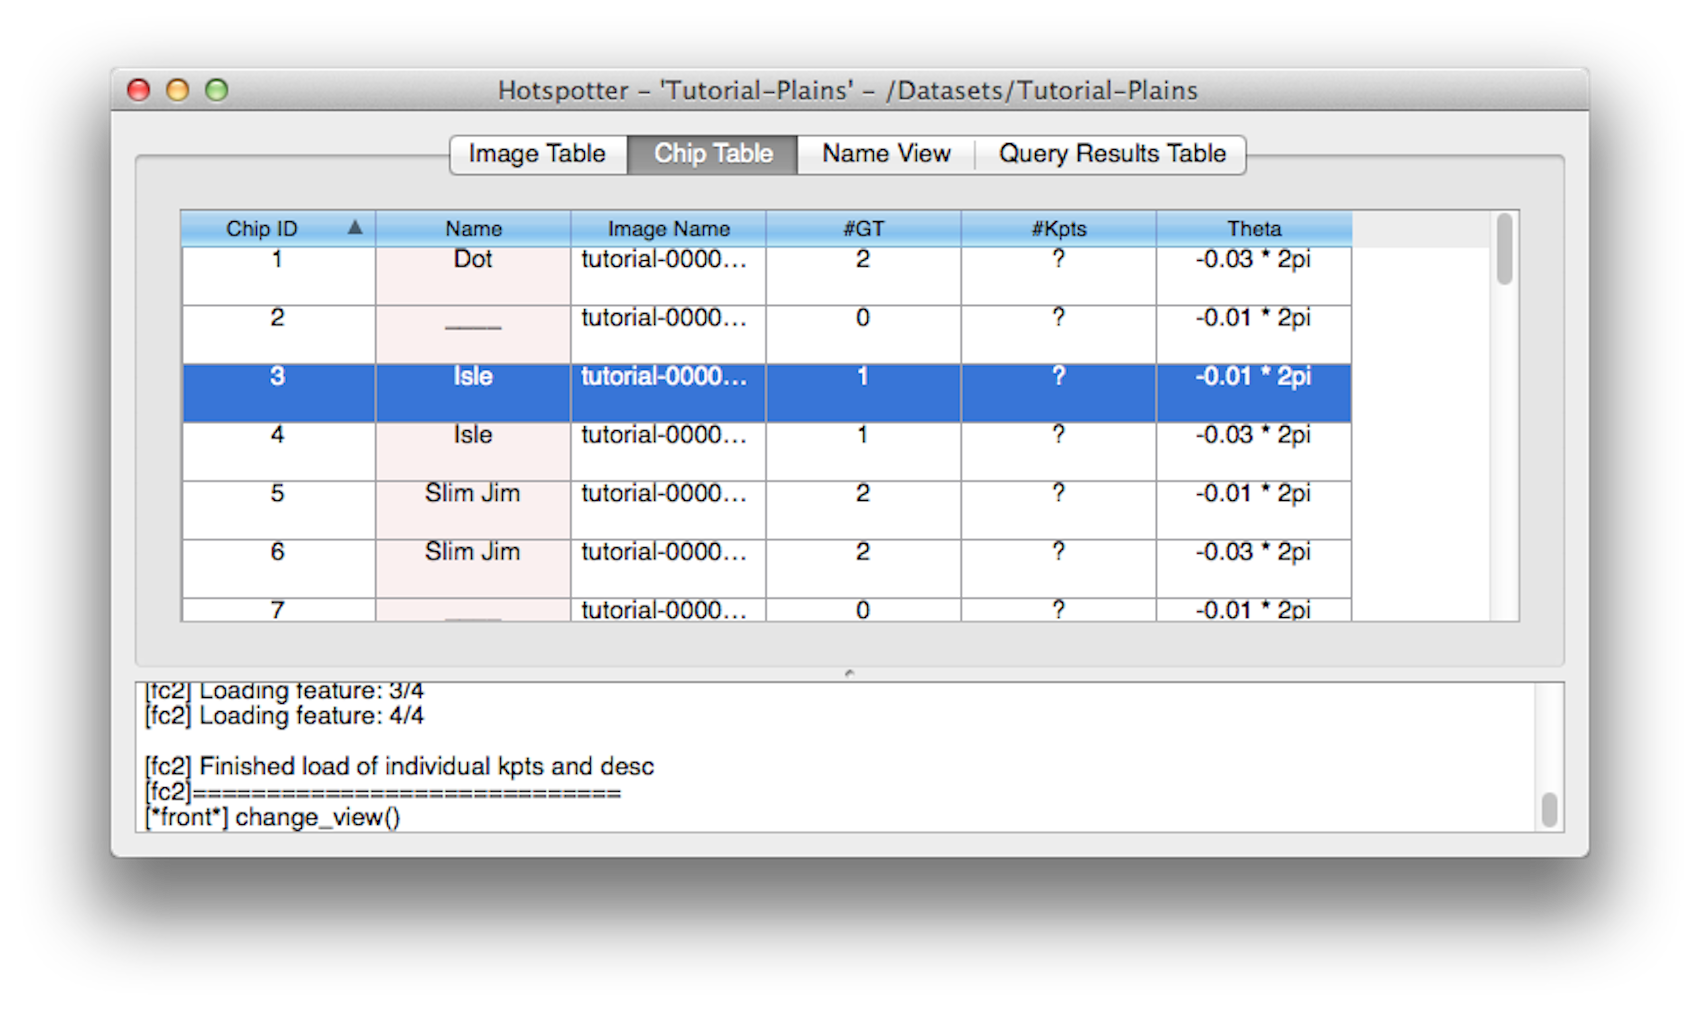
\includegraphics[scale=0.1]{images/names.png}
            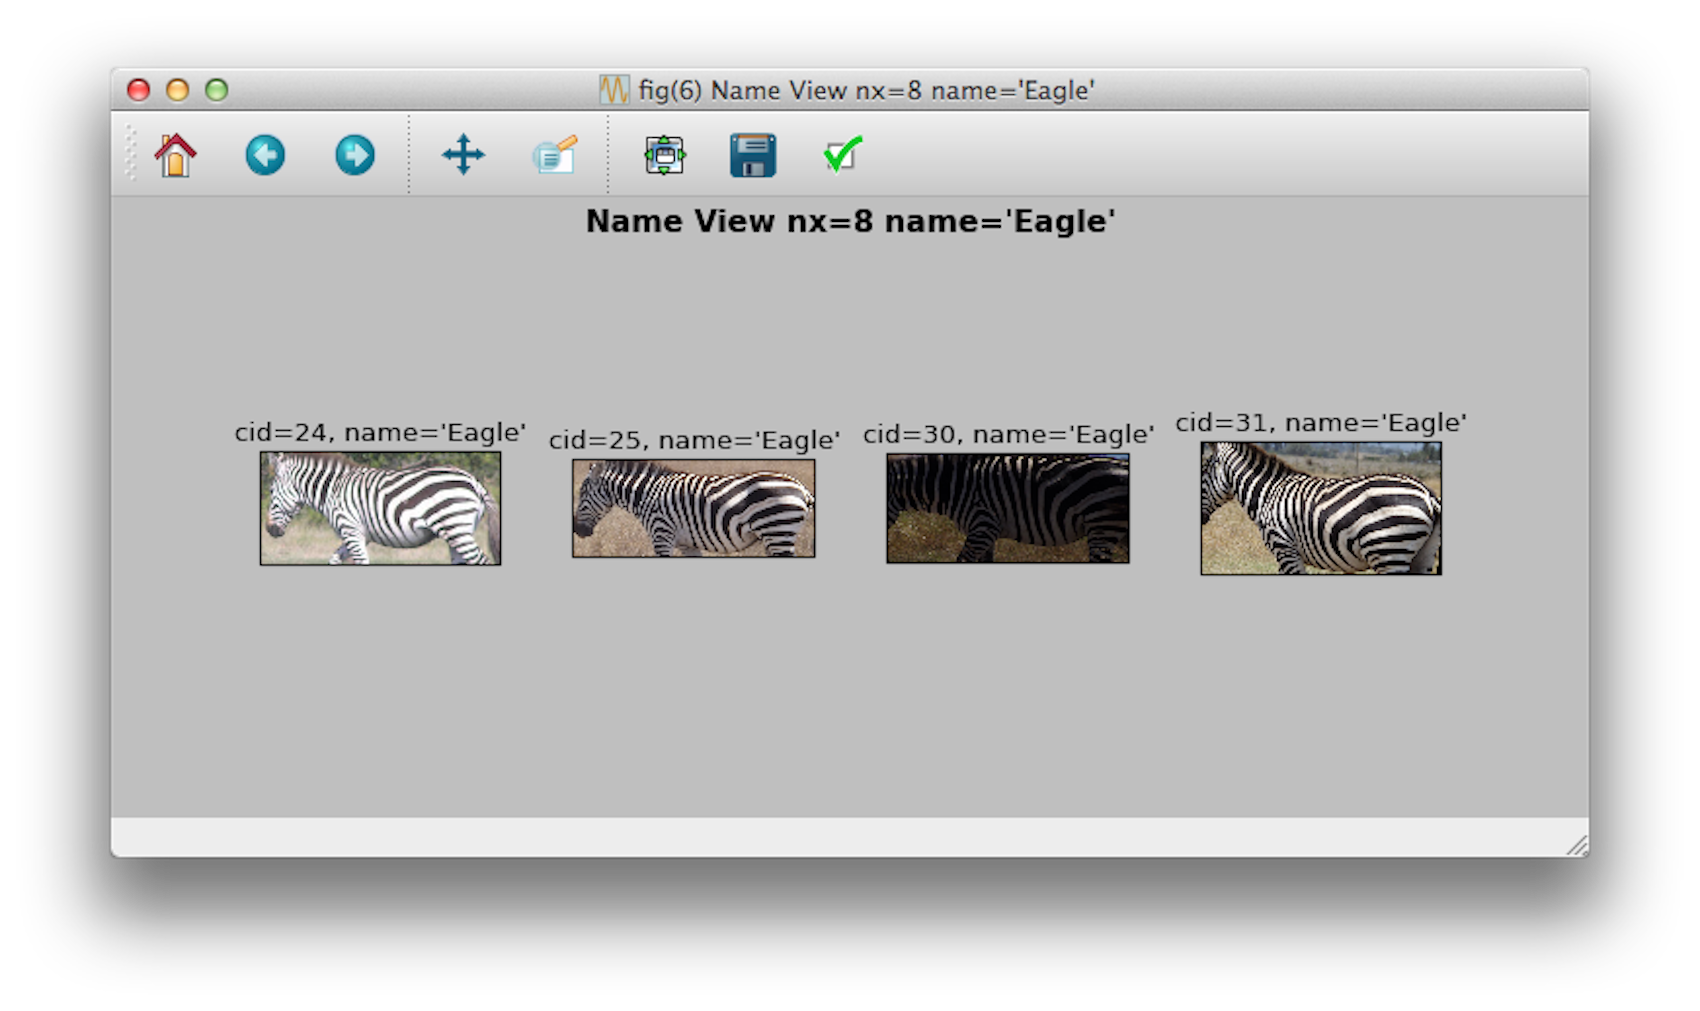
\includegraphics[scale=0.1]{images/matches.png}
\end{center}

\noindent
  The Chip ID is the unique numerical index HotSpotter applies to
  each chip.  (Remember, there can be more than one ROI/chip per image.)
  As HotSpotter does its work and chips are successfully matched,
  users will want to assign names to individual animals and use this
  same name for all chips in which the animal appears.  Initially,
  before an image is recognized, the ``Name'' column value will
  be specified as ``\_\_\_\_'' (four underscores).  This denotes an
  unidentified chip - a user may double-click on a name to edit. 
  To view animals that match, simply go to the Name View to view all of the matched objects with the same name. 
  Use of copying and pasting from one chip name to the other makes this process less prone to
  typing errors.



\section{Additional Tools and Tricks}


Here is a brief discussion of are a few additional tricks and options
for running HotSpotter:
\begin{itemize}
\item \verb+Actions -> Select Next+:
    selects either the next image that does not already have an ROI or the next chip without an
    orientation. 

\item \verb+Actions -> New Chip Property+:  
    record metadata as a series of one or more attribute/value pairs for any
    user defined metadata.  HotSpotter will automatically import existing
    metadata from StripeSpotter databases.


%\item \verb+Options -> Toggle Plot Widget+: 
    %shows the results plot in a separate pane.  This is particularly useful for
    %resizing the pane when there are many results.

\item \verb+Options -> Edit Preferences+: 
    change the behavior of HotSpotter. For now, these are not very well
    documented and should only be used with specific guidance from 
    the HotSpotter team.

%\item \verb+Convenience -> Convert All Images to Chips+: 
    %make each image its own ROI and therefore image chip.

%\item \verb+Convenience -> Batch Change Name+:  
    %change all chip instances of a given name to a new name. This is useful for
    %when the same animal is grouped under two different names.

%\item \verb+Convenience -> Assign Matches Above Threshold+: 
    %HotSpotter will automatically run each chip in the database as a query and
    %assigns it as a match to any chips whose matching score is above a
    %user-define threshold. 

\item \verb+Help -> View Data Directory+: 
    Opens the current database directory.

\item \verb+Help -> View Source Directory+: (primarily for developer usage)
    Opens the HotSpotter source directory. 

\item \verb+Help -> View Internal Directory+: 
    Opens the current database's {\tt \_hsdb} directory

\item \verb+Help -> Delete Computed Directory+: 
    Removes all of HotSpotter's internal cache. It should be used if you suspect
    the database has been corrupted. This forces everything to be recomputed. 

\item \verb+Help -> Delete Global Preferences+: 
    This resets hotspotters external preferences. You may need to do this if you
    are upgrading versions. 
    %This removes HotSpotter's external cache, which may have inconsistent
    %file formats between versions. If HotSpotter has trouble loading try this
    %first. 

%\item \verb+Matching Experiment+: (primarily for developer usage)
    %Runs an experiment to see what matches HotSpotter assigns to each chip.
    %Output is written to the database directory. 

%\item \verb+Run Name Consistency Experiment+: (primarily for developer usage) 
    %Runs an experiment to see if HotSpotter agrees with the current labeling.
    %Output is written to the database directory. 

\end{itemize}
  


\section{A Bit of Troubleshooting}

In the event that HotSpotter behaves unexpectedly, the first thing to try is a
restarting the program. If the error persists, the following will fix common
errors: 

\begin{itemize}
    \item \textbf{Delete your preference directory.}\\
        HotSpotter keeps a small set of preference files in the user's  home directory.
        These files remember the last database opened as well as other
        preferences. When updating to new versions these can sometimes cause
        problems. Deleting the {\tt \texttildelow/.hotspotter}\footnote{Note
            that {\tt \texttildelow} denotes the user's home folder} folder may fix some issues.\\

    \item \textbf{Re-Import the Images}\\
        If the images you've imported aren't showing up, you can always re-import
        the images in\\ {\tt user\_database\_dir/images}
        directory. (REALLY???  THIS DOES NOT CREATE PROBLEMS???)  \\

    \item \textbf{Delete the Computed Directory}\\
        If something looks corrupted or ROIs are being oddly drawn, the user
        should consider deleting the computed directory.  Running  the command 
        {\tt (Convenience \textrightarrow{} View Internal Directory)} will open
        {\tt user\_database\_dir/\_hsdb} directory. From here the
        {\tt computed} directory may be deleted. This will cause the program
        to recompute all of its data. The user may have to restart HotSpotter.\\


    \item (UPDATE ME!!!!!)  \textbf{Mac OSX 10.8 Gatekeeper}\\ For Mac OSX 10.8 Mountain
      Lion users this app might not run.  This error is due to a
      security feature within Mountain Lion called Gatekeeper.  If the
      app fails to run, please do the following:
        \begin{enumerate}
            \item Go to {\tt System Preferences} --- Click the Apple icon in the menu bar (top-left of the screen) and select {\tt System Preferences} in the drop down menu.
            \item Go to {\tt Security \& Privacy} --- It is located on the top row, entitled {\tt Personal}.
            \item Go to the {\tt General} tab.
            \item Authenticate --- Click on the lock at the bottom-left corner of the screen and subsequently input your computer username and password.
            \item In the bottom half of the {\tt General} tab, there will be the following selection:
                \begin{Verbatim}
                    Allow applications downloaded from:
                    ( ) Mac App Store
                    (X) Mac App Store and identified developers
                    ( ) Anywhere

                \end{Verbatim}

                Select {\tt Anywhere} and subsequently select {\tt Allow From Anywhere} in the drop down warning.

            \item Close the {\tt System Preferences} window.
            \item Install HotSpotter and run it.
            \item To re-enable security after running HotSpotter once,
                repeat the above changes to your preferences, except click on
                \texttt{Mac App Store and identified developers}.
        \end{enumerate}


    \item \textbf{Email the Developer}\\
        If all else fails users should send an email to \developeremail{}.
        Please include a detailed description of the error and what was being done when it
            happened.  Then also please copy the text in the output window to a text file, and include this in your email.\\
    \end{itemize}

%\section{Source Code Dependencies}
%
%The remainder of this discussion only applies to downloading and
%working with the source code instead of the installer packages.
%
%Before executing HotSpotter from the source code users should ensure
%that their environment is set up correctly. Primarily, this includes
%Python 2.7.3, Qt, and OpenCV, but it also includes several supporting
%packages.  Users who want to use HotSpotter without modification
%should download the installer package instead.
%
%    \subsection{Windows}
%        Install the following dependencies in order.  
%        \textbf{The software is untested using 64-bit python. It is preferred to use 32-bit builds of each dependency when specified.}
%        \begin{enumerate}
%            \item Python 2.7 32-bit
%                \begin{enumerate}
%                    \item Download:
%                        \url{http://www.python.org/download/releases/2.7.5/}
%                    \item Install with install packager
%                \end{enumerate}
%
%            \item MinGW (C / C++) 
%                \begin{enumerate}
%                    \item Download: 
%                        \url{http://sourceforge.net/projects/mingw/files/latest/download?source=files}
%                    \item Install with install packager
%                    \item REQUIRED: C and C++ COMPILER
%                \end{enumerate}
%
%            \item Qt Library 4.8 32-bit 
%                \begin{enumerate}
%                    \item Download: \url{http://qt-project.org/downloads}
%                    \item Install with install packager
%                \end{enumerate}
%
%            \item PyQt4 32-bit 
%                \begin{enumerate}
%                    \item Download:
%                        \url{http://www.riverbankcomputing.com/software/pyqt/download}
%                    \item Install with install packager
%                \end{enumerate}
%
%            \item NumPy 32-bit 
%                \begin{enumerate}
%                    \item Download:
%                        \url{http://sourceforge.net/projects/numpy/files/NumPy/1.7.1/numpy-1.7.1-win32-superpack-python2.7.exe/download}
%                    \item Install with install packager
%                \end{enumerate}
%
%            \item matplotlib 32-bit 
%                \begin{enumerate}
%                    \item Download: \url{http://matplotlib.org/downloads.html}
%                    \item Install with install packager
%                \end{enumerate}
%
%            \item PIL 32-bit 
%                \begin{enumerate}
%                    \item Download:
%                        \url{http://www.pythonware.com/products/pil/}
%                    \item Install with install packager
%                \end{enumerate}
%        \end{enumerate}
%        \;
%
%    \subsection{Mac OSX}
%
%        Install the following dependencies in order.
%        \begin{enumerate}
%
%            \item Qt Library 4.8 
%                \begin{enumerate}
%                    \item Download: \url{http://qt-project.org/downloads}
%                    \item Install with install packager
%                \end{enumerate}
%
%            \item XQuartz - This dependency is required for FreeType
%                (\url{http://www.freetype.org/}) and libpng
%                (\url{http://www.libpng.org/pub/png/libpng.html}) 
%                \begin{enumerate}
%                    \item Download: \url{http://xquartz.macosforge.org}
%                    \item Install with install packager
%                \end{enumerate}
%
%            \item SIP 
%                \begin{enumerate}
%                    \item Download:
%                        \url{http://riverbankcomputing.co.uk/software/sip/download}
%                    \item sudo python configure.py
%                    \item sudo make
%                    \item sudo make install
%                \end{enumerate}
%
%            \item PyQt4 
%                \begin{enumerate}
%                    \item Download:
%                        \url{http://www.riverbankcomputing.com/software/pyqt/download}
%                    \item sudo python configure.py
%                    \item sudo make
%                    \item sudo make install
%                \end{enumerate}
%
%            \item NumPy 
%                \begin{enumerate}
%                    \item Download:
%                        \url{http://sourceforge.net/projects/numpy/files/latest/download?source=files}
%                    \item sudo python setup.py install
%                \end{enumerate}
%
%            \item matplotlib 
%                \begin{enumerate}
%                    \item Download: \url{http://matplotlib.org/downloads.html}
%                    \item sudo python setup.py install
%                \end{enumerate}
%
%            \item libjpeg 
%                \begin{enumerate}
%                    \item Download: \url{http://www.ijg.org/}
%                    \item ./configure
%                    \item sudo make
%                    \item sudo make install
%                \end{enumerate}
%
%            \item PIL 
%                \begin{enumerate}
%                    \item Download:
%                        \url{http://www.pythonware.com/products/pil/}
%                    \item sudo python setup.py install
%                \end{enumerate}
%        \end{enumerate}
%        \;
%

\section{Source Code}

    \subsection{License}
HotSpotter is currently distributed under the Apache License, Version 2.0.
\begin{Verbatim} 
   HotSpotter
   Copyright © 2014 Jon Crall, Jason Parham, Chuck Stewart
   Department of Computer Science 
   Rensselaer Polytechnic Institute

   Licensed under the Apache License, Version 2.0 (the "License");
   you may not use this file except in compliance with the License.
   You may obtain a copy of the License at

       http://www.apache.org/licenses/LICENSE-2.0

   Unless required by applicable law or agreed to in writing, software
   distributed under the License is distributed on an "AS IS" BASIS,
   WITHOUT WARRANTIES OR CONDITIONS OF ANY KIND, either express or implied.
   See the License for the specific language governing permissions and
   limitations under the License.


\end{Verbatim}

\subsection{Download}
Download the source code here: \url{https://github.com/Erotemic/hotspotter}
\begin{Verbatim}[commandchars=\\\{\}]
git clone git@github.com:Erotemic/hotspotter.git
\end{Verbatim}

%Users will also need to check out the tpl submodule.  This can be be
%done separately, or by running the command: 
%\begin{Verbatim}[commandchars=\\\{\}]
%python setup.py configure
%\end{Verbatim}
%This will also ensure that files have the correct permissions. 

Once the source code has been downloaded the program can be run by using the command:
\begin{Verbatim}[commandchars=\\\{\}]
./main.py
\end{Verbatim}

        %To build the program into a Windows .exe, execute the command:
        %\begin{Verbatim}
        %python setup.py py2exe
        %\end{Verbatim}

        %To build the program into a Mac .app, execute the command:
        %\begin{Verbatim}
        %python setup.py py2app
        %\end{Verbatim}

\subsection{Contribute}
HotSpotter is an open source project. If any tech-savvy users develop a cool
feature or a bug-fix and would like to see it incorporated, send an email with the proposed
patch to \developeremail{} for code review.

\newpage



\end{document}
